% Chapter Template

\chapter{Background} % Main chapter title

\label{Chapter2} % Change X to a consecutive number; for referencing this chapter elsewhere, use \ref{ChapterX}

In this chapter, we will introduce some necessary background knowledge in order to let the reader understand better how this project came into its form.

Not only the technology stack that this project used is important to further understanding, but also some theoretical part that's behind. We shall introduce it gradually.

%----------------------------------------------------------------------------------------
%	SECTION
%----------------------------------------------------------------------------------------

\section{Web Technology Stack}

Before starting to program on the software that shows the different ways to show an interface providing \gls{fpc} with many \gls{lod}, we must first choose the nature and language of the program. A web technology stack program stands out easily and as a matter of fact, was also the first choice for the development of the immature prototype in the first place. There are several reasons behind it. For web technology stack developed programs:

\begin{itemize}
    \item \textbf{Compatibility} Code once, it works everywhere. It saves lots of time for users and testers to read a long manual. All we need is a working browser with loose requirements to it.
    \item \textbf{Simple Installation} Almost nothing to be installed in order to see the project up and running. Besides a browser of some version specifications, only a web server of \emph{any kind} is required, as described in \gmref{chap4:starttheproject}.
    \item \textbf{Appearance} Can look modern with almost zero code. Can have cool visual effects a lot easier than desktop development. 
    \item \textbf{Successful Case} If it works for Google Maps, it should work for our project as well.
    \item \textbf{Performance} Slower in a sense because hardware resources are not easily fetched for browser-based \gls{ui} heavy applications.
\end{itemize}

On the other hand for desktop development:

\begin{itemize}
    \item \textbf{Compatibility} Really common to be ``working on my computer'' but not on users'.
    \item \textbf{Simple Installation} Lots of preconditions and require lots of planning before the delivery of a standalone package. If not planned and all aspects chosen carefully, applications might not work on Macs and gives pop-ups to require ``vcredist'' dependencies on other operating systems.
    \item \textbf{Appearance} Requires lots of coding to have the most basic appearance. Visual effects need to be programmed manually one by one, not to mention the planning of the software structure. 
    \item \textbf{Successful Case} Works also fine with lots of deep zooming applications such as \emph{Ultra Fractal} and \emph{Kalles Fraktaler}.
    \item \textbf{Performance} Can be a lot faster than web applications if choosing \emph{C} / \emph{C++} or similar languages since they can access directly your hardware resources.
\end{itemize}

Since this project is focused a lot on the front end \gls{ui}, web technologies is chosen even when performance can sometimes hinder the advancement of some applications. If planned well, performance on the deep zooming part of the project can be improved by coding techniques and algorithms, however, on the other hand, programming front end \gls{ui} effects together with planning a good structure to use the advantages of calculation speed of desktop applications would not be productivity efficient.

\glsunset{gpu}
\glsunset{cpu}

Some other approaches were also considered, for example to use an intermediate solution like Python because it can be easily structured and coded, however, most of them were not as good choices as web technologies. Taking Python as an example, it cannot do conventional iterations over pixels fast enough unless complicated techniques are used, which actually brings it back on the same level with desktop programming, not to mention the invocation of hardware \gls{gpu} / \gls{cpu} resources and fast image manipulations --- they all bring lots of complications to the implementation of the project.

%----------------------------------------------------------------------------------------
%	SECTION
%----------------------------------------------------------------------------------------

\section{Web, HTML5 And Canvas API}

After the choice of web technology stack, we'll be talking about the equipments that are used in the project.

Technically speaking, web wechnologies are focused on \gls{ui} and communications between servers and computers since the computers and servers on the internet can't communicate with each other the way people do, however, the communication part is not hugely focused in this project. First thing to know is that web technology stack includes the markup languages and multimedia packages servers and computers use to communicate, however, it's the markup languages and multimedia packages that we focus on, not the communication part, since the communication involved currently is still on local machines.

\subsection{Browsers}

Web technology runs on browsers. Browsers are the tools that request information and then they show us users in the way we can understand, as the interpreters of the web programs. There are many famous web browsers around:

\begin{itemize}
    \item \textbf{Google Chrome} Currently the most popular browser by Google
    \item \textbf{Safari} Apple's web browser
    \item \textbf{Firefox} Open-source browser supported by the Mozilla Foundation
    \item \textbf{Internet Explorer} Microsoft's browser
\end{itemize}

And since Google Chrome has the most popularity and supports all of our requirements for the project, we chose Google Chrome as our browser for the project.

\subsection{Markup Language}

There are some fundamental things for web programming. The first things we need to know about are \gls{html}, \gls{css} and \gls{js}.

\paragraph{HTML}

\gls{html} is one of the first thing to be introduced in this section. Thanks to \gls{html}, the browsers can know what to present when we hit them we a request. It is the standard markup language for documents designed to be displayed in a web browser. It can be assisted by technologies such as \gls{css} and scripting languages such as \gls{js}.\cite{wiki:html}

\paragraph{CSS}

\glsreset{js}

The technology assisting \gls{html} describes how \gls{html} elements are to be displayed on the screen, if to be put straightforward. It is a style sheet language used for describing the presentation of a document written in a markup language like \gls{html}.\cite{wiki:css} \gls{css} is a cornerstone technology of the web technologies, alongside \gls{html} and \gls{js}.\cite{flanagan2006javascript}

\paragraph{JavaScript}

\glsreset{js}

Alongside \gls{html} and \gls{css}, \gls{js} is one of the core technologies of the World Wide Web.\cite{flanagan2006javascript} JavaScript enables interactive web pages and is an essential part of web applications. The vast majority of websites use it,\cite{w3techs2018usage} and major web browsers have a dedicated JavaScript engine to execute it.\cite{wiki:js}

\subsection{HTML5}\label{chap2:html5}

It is worth mentioning that there is more to the technologies this project is using than the traditional \gls{html} / \gls{css} / \gls{js}, which is the larger set --- \gls{h5}. \gls{h5} is the latest evolution of the standard that defines the original. The term \gls{h5} represents two different concepts:

\begin{itemize}
    \item It is a new version of the markup language \gls{html}, with new elements, attributes, and behaviors
    \item A larger set of new web technologies that allows the building of more diverse and powerful applications.
\end{itemize}

Therefore, this set is sometimes called \emph{\gls{h5} and friends} and often shortened to just \gls{h5}.

There are lots of new features that \gls{h5} brings to the original \gls{html}, but we're not describing all them there in full\footnote{ See \url{https://en.wikipedia.org/wiki/HTML5} to know more details}. The core features we care about and using in this project are the following two:

\paragraph{Graphics and Effects} Allowing a much more diverse range of presentation options, with respect to 2D / 3D graphics and effects.
\paragraph{Performance and Integration} Providing greater speed optimization and better usage of computer hardware.
\paragraph{Styling} Allowing more sophisticated themes and \gls{ui} experience.

Solving exactly the problems of our focus points in this thesis. Some more specific details to each of the above points and their applications in this project will be shortly described.

In the graphics part, the new element \texttt{<canvas>} element that allows delicate drawing on web pages are heavily used. 

In the performance and integration part, \emph{Web Worker}s are used allowing delegation of \gls{js} evaluation to background threads, preventing these operations from slowing down \gls{ui} interactive events. The separation used in the project can also be easily advanced by replacing this multithreading calculation part with the new \emph{XMLHttpRequest} allowing fetching information asynchronously, also allowing it to display dynamic content, varying according to the time and user actions\footnote{ This is the technology behind \emph{Ajax}. To know more information about \emph{Ajax}, see \url{https://en.wikipedia.org/wiki/Ajax_(programming)}.}. 

In the styling part, since the new \gls{css} in \gls{h5}, \gls{css3}, has been extended to be able to style elements in a much more complex way, many new features of \gls{css3} are used, such as:

\paragraph{Background Styling}

The possibility to put shadows on elements using \texttt{box-shadow} and \gls{css} \texttt{filter}s. These advanced box effects are used in this project for the display of halos of the context views and also internally in the dependencies of this project, \emph{jQuery}\footnote{ jQuery is an open-source, fast, small, and feature-rich JavaScript library. It makes things like HTML document traversal and manipulation, event handling, animation, and Ajax much simpler with an easy-to-use API that works across a multitude of browsers. See \url{https://jquery.com/} for more information.} and \emph{Bootstrap}\footnote{ Bootstrap is an open source toolkit for developing with \gls{html}, \gls{css}, and \gls{js}. See \url{https://getbootstrap.com/} for more information.}.

\paragraph{Animating of Styles}

Using CSS Transitions to allow the animation between different states or using \emph{\gls{css} Animations} to animate parts of the page without a triggering event, for example some movement animations of the context views in this project.

\paragraph{New Presentational Layouts}

Two new layouts have been added to \gls{css3}: the \gls{css} multi-column layouts and \gls{css} flexible box layout, and the latter is used in multiple places in this project, for example, the default layouts for the context views and the tabs layouts for the conext views. The dependency \emph{Bootstrap} also relies largely on this new feature.

\subsection{Canvas API}

\gls{h5} brought exciting new advantages to the \gls{html} coding world as mentioned above. Amongst them all, one of the most thrilling one, the new \texttt{<canvas>}, allows us to render delicate graphics powered by \gls{js}. We'll be talking about what it is and then the \gls{api} that supports its usages.

\texttt{<canvas>} is an \gls{html} element which can be used to render graphics via scripts\footnote{ To know about the \texttt{<canvas>} element, see \url{https://en.wikipedia.org/wiki/Canvas_element}.}, here in our project \gls{js}. It can, for instance, be used to draw graphs or create simple (and not so simple) animations. In our project, \texttt{<canvas>} is used for the graphical representation of the extreme resolution datasets.

It's also worth mentioning that after first introduced in \emph{WebKit} by \emph{Apple} for the \emph{OS X Dashboard}, \texttt{<canvas>} has since been implemented and supported in all major browsers today.

The Canvas \gls{api} itself is a sense of how to use scripts to draw on this newly introduced \gls{html} element. It is largely focuses on 2D graphics. The reason to bring it up here together with the \texttt{<canvas>} element is that there are many other \gls{api}s that come together with it, for example the WebGL \gls{api}, which also uses the \texttt{<canvas>} element, draws hardware-accelerated 2D and 3D graphics. In another word, the context of the \texttt{<canvas>} element\footnote{ Here not the same concept as the ``context'' in the previously mentioned term \gls{fpc}.} is ``2d'' through the Canvas \gls{api}, not ``webgl'' context or any other.

%----------------------------------------------------------------------------------------
%	SECTION
%----------------------------------------------------------------------------------------

\section{Mandelbrot Set}

As for the datasets themselves, we use a kind of computable dataset instead of a static and deep zoomable image information dataset. The advantage is obvious that by using a dataset that can be computed for its information of any specific point in the set, we don't have to store the information anywhere anymore, as if we did, it would require a lot of investment and investigation for the storage or fetching of the dataset for this project. The downside of it is also clear that we'll have to trade time for space, since the calculation is usually going to take more time than only querying from a static set of data. It is proved to be solid to do this trade, since in this project, the visually inspected results shows that the waiting time is still inside human tolerable margins.

The dataset we chose is the Mandelbrot set. The Mandelbrot set is a famous example of a fractal in mathematics. It is named after Beno\^{\i}t Mandelbrot, a Polish-French-American mathematician\footnote{ Its definition and name are due to Adrien Douady, in tribute to the mathematician Beno\^{\i}t Mandelbrot\cite{wiki:mandel}.}. The reason this thesis is using Mandelbrot set as the source of extreme resolution dataset is because Mandelbrot set can provide theoretically infinitely high resolution datasets. In this section, we'll introduce briefly Mandelbrot set, its algorithms ideas for visualization.

\subsection*{What Is Mandelbrot Set}

Firstly, we recursively define a sequence $\displaystyle (z_{n})_{n\in\mathbb{N}},\thickspace z_{n}\in\mathbb{C}$ as follows:

\begin{equation}
    z_0 = 0
\end{equation}

\begin{equation}
    z_{n} = z_{n-1}^2 + c,\thickspace c\in\mathbb{C}
\end{equation}

For different constant $c$, the absolute value of $z_n$ could remain bounded, could also be divergent, if $n$ is increased.

The Mandelbrot set $\mathbb{M}$ is the set of $c$ in the complex plane for which the sequence $\displaystyle (z_{n})_{n\in\mathbb{N}},\thickspace z_{n}\in\mathbb{C}$ remains bounded.

\subsection*{Important Properties of the Mandelbrot Set}

A property of Mandelbrot set is as follows:

A complex number $c$ belongs to the Mandelbrot set $\mathbb{M}$, if and only if the absolute value of $z_n$ is not larger than $2$, for all $n = 0, 1, 2, ..$

\subsection*{Simple Graphical Presentation}

The following figure \gmref{fig:mandelbrot} is a simple graphical representation of Mandelbrot set. A point $c$ in the complex plane is conventionally colored \emph{black} if it belongs to the Mandelbrot set $\mathbb{M}$, and \emph{white} if not. 

\begin{figure}[th]
\centering
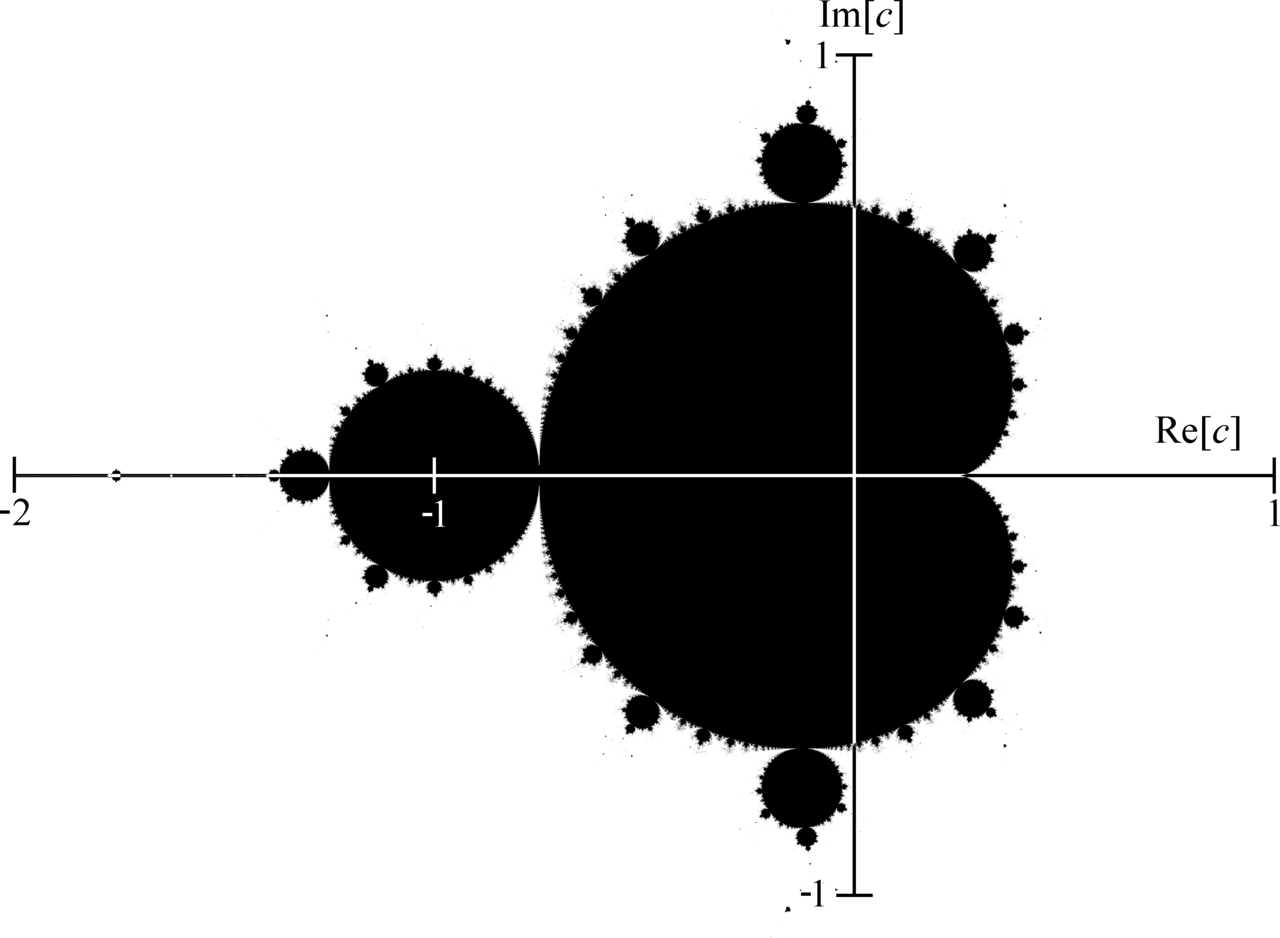
\includegraphics[width=\textwidth,keepaspectratio]{Figures/Chapter2/mandelbrot.png}
% 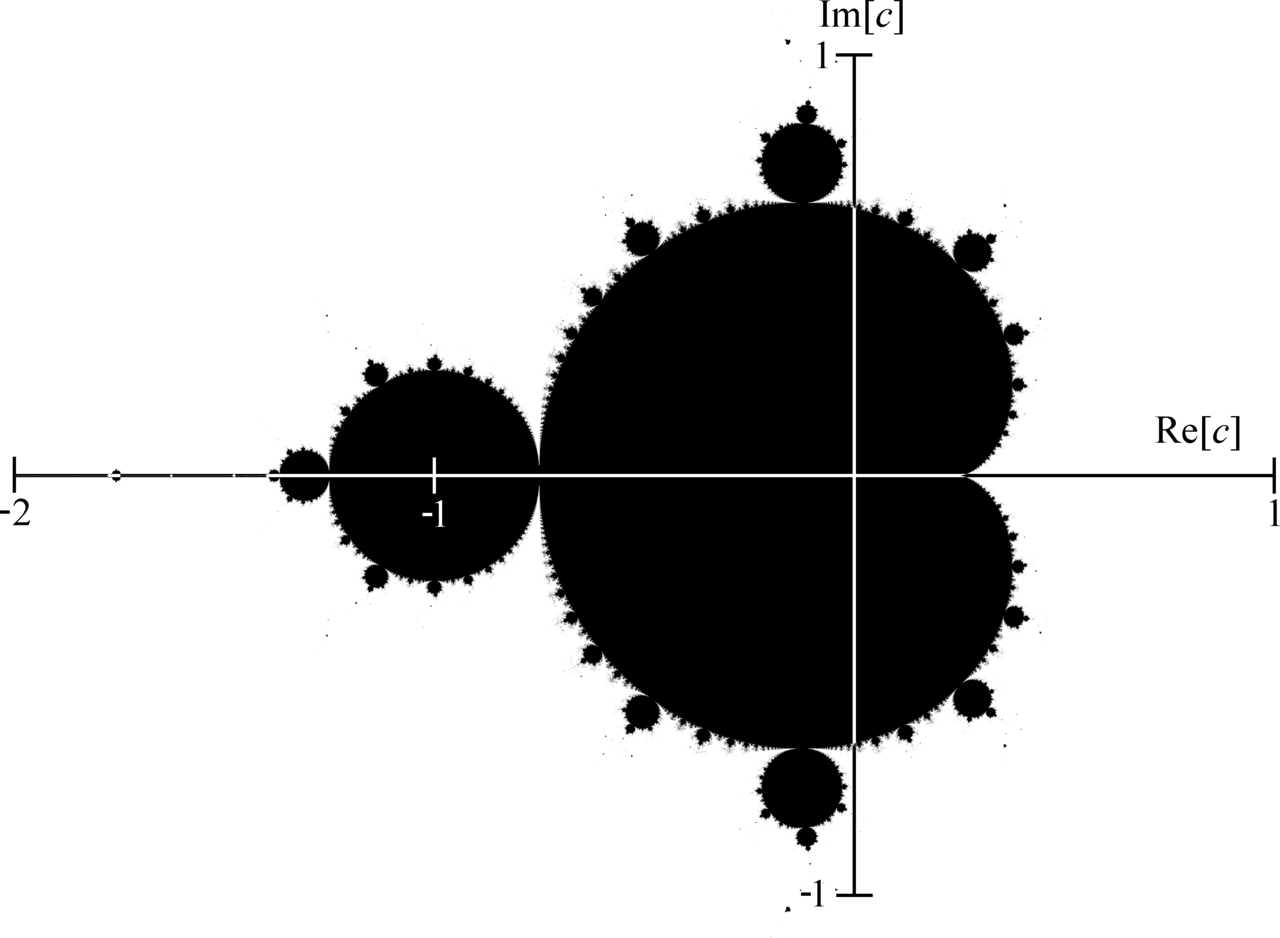
\includegraphics{Figures/Chapter2/mandelbrot.png}
\decoRule
\caption[Mandelbrot Set Graphical Presentation]{A simple graphical representation of Mandelbrot set.}
\label{fig:mandelbrot}
\end{figure}

\subsection*{Algorithms for Visualization}\label{chap2:algorithmsforvisualization}

A simple algorithm is introduced for visualization of black and white in \gmref{alg:simple}.

\begin{algorithm}[H]
    \ForEach{$c$ in complex plane}{
        $z_0 = 0$\;
        \For{$n \leftarrow 0$ \KwTo $max$}{
            $z_n = z_{n - 1}^2 + c$\;
            \If{the value of $z_n$ is larger than $2$}{
                $c$ does not belong to $\mathbb{M}$. In this case, we set the color of $c$ to \emph{white} and the calculation of sequence is stopped\;
            }
            \uElseIf{$n = max$}{
                $c$ belongs to $\mathbb{M}$ and we set the color of $c$ to \emph{black}\;
            }
        }
    }
    \caption{Algorithms for Simple Visualization}
    \label{alg:simple}
\end{algorithm}

In \gmref{alg:simple}, the variable $max$ can be treated as a constant for each complete cycle of the execution of the algorithm. The larger $max$ is, the more accurate the image generated will be. However, it should not be set infinitely large as a point belonging to the Mandelbrot set will cause the algorithm to loop infinitely. A simple equation is used for the determination of this value $max$:

\begin{equation}
    \label{eq:max}
    {(50 \cdot log_{\thinspace 10 \thinspace}{magnif})}^{1.08}
\end{equation}

Where $magnif$ is the magnification level, a number representing the number of pixels that together has a length of $1$ on the mathmatical axis, shown in \gmref{fig:magnif}.

\subsection*{Algorithms Idea for Graphical Representation with Grayscale}

In the mentioned algorithm \gmref{alg:simple}, $c$ is set to either \emph{black} or \emph{white}. If the iteration number $n$ is equal to the maximum iteration number $max$ and the value of $z_n$ still less than $2$, then $c$ has the color \emph{black}. If the iteration number $n$ is smaller than $max$ then at this moment the absolute value of $z_n$ becomes larger than $2$. In this case, we cannot set the color of $c$ to \emph{black}, because $c$ dose not belong to Mandelbrot set. However, we set a color with a portion of \emph{black}, to indicate how close $c$ is to be in \emph{black} area, as shown in \gmref{alg:grayscale}.

\begin{algorithm}[H]
    \ForEach{$c$ in complex plane}{
        $z_0 = 0$\;
        \For{$n \leftarrow 0$ \KwTo $max$}{
            $z_n = z_{n - 1}^2 + c$\;
            \If{the value of $z_n$ is larger than $2$}{
                $c$ does not belong to $\mathbb{M}$\;
                In this case, we set the color of $c$ to \st{\emph{white}} \emph{grayscale\footnote{ In the current implementation, this color is set to be grayscaled red, rgb($grayscale\% \times 255$, 0, 0).} depending on the number of iteration} $n$ and the calculation of sequence is stopped\;
            }
            \uElseIf{$n = max$}{
                $c$ belongs to $\mathbb{M}$ and we set the color of $c$ to \emph{black}\;
            }
        }
    }
    \caption{Algorithms for Grayscale Visualization}
    \label{alg:grayscale}
\end{algorithm}

The value $max$ is determined in the same way as described in \gmref{eq:max}.